\chapter{Flujo de Diseño Digital de Circuitos Integrados con las herramientas de Synopsys. Estructura de Scripting}
\label{ch:solucion}

% Primero que todo, jamás utilice el título indicado arriba, sino algo
% relacionado con su solución: ``Sistema de corrección de distorsión'' o lo que
% competa a su tesis en particular.

% Este capítulo puede separarse en varias secciones, dependiendo del problema
% concreto. Aquí los algoritmos o el diseño del sistema deben quedar lo
% suficientemente claros para que otra persona pueda re-implementar al sistema
% propuesto. Sin embargo, el enfoque no debe nunca concentrarse en los detalles
% de la implementación particular realizada, sino del diseño conceptual como tal.

% Recuerdese que toda figura y tabla deben estar referenciadas en el texto.

A continuación se detalla la estructura propuesta para implementar un flujo de diseño de circuitos integrados, y se expone como fueron sometidos los módulos de un microprocesador ASP RISC-V, con el fin de demostrar la efectividad del flujo de diseño digital propuesto. Esta estructura está basada en el manual sobre el uso de las herramientas de Synopsys en el flujo de diseño de ASICs, del Instituto Tecnológico de Costa Rica \cite{FlujoJairo2016}.

La siguiente estructura dista considerablemente de la propuesta en \cite{FlujoJairo2016} y que a su vez está basada en el manual \cite{kommuru2009asic}. En estos trabajos las estructuras se basan en ejemplos simples con diseños \textit{HDL} relativamente pequeños. La siguiente estructura toma como premisa que se trabaja con diseños muy grandes por lo que se requiere de mayor eficiencia en la generación de las bases de datos y archivos necesarios para el diseño.

Dado que las herramientas EDA que se utilizan corren en "Linux", muchos de los scripts que se encuentran en esta estructura, hacen referencia a particularidades de este sistema operativo y no se describen en detalle pues abundar sobre el entorno "CentOS de Linux" esta fuera del objetivo de este proyecto, es por ello que se parte de la premisa que el lector cuenta con el conocimiento suficiente de este sistema operativo.

La primera propuesta de esta estructura fue desarrollada por el Dr. Juan Agustín Rodríguez y se tomó como referencia para desarrollar la que a continuación se expondrá. La estructura que se propone se basa en 3 principios muy relacionados con el mundo de desarrollo de software; sin embargo, apelan más a la experiencia práctica del Dr. Rodríguez y del aspirante que escribió este informe.

\begin{itemize}
\item {\textbf{Regularidad:}} {Este concepto se refiere a la uniformidad con la que los elementos desarrollados se ubican, dentro de la estructura de archivos y directorios, los cuales están basados en un principio o plan.

Esta estructura es "regular" en tanto presenta la misma morfología para los distintos directorios, esto quiere decir que aunque los directorios contienen archivos de distinta naturaleza, la mayoría presentan una jerarquía constante entre sí.}

\item {\textbf{Localidad:}} {Se refiere a usar archivos y directorios únicos, para evitar el manejo de múltiples versiones y múltiples rutas de acceso a archivos que en esencia son iguales, lo cual suele ser un problema cuando se debe involucrar a más personas en un proyecto.

La estructura presenta "localidad" en tanto los archivos fuente y las bases de datos generadas por los procesos de síntesis, únicamente residen en un único directorio y presentan sólo una ruta de acceso, no se generan copias de estos archivos en otros directorios, y la forma en que se accede a ellos es mediante punteros. Existen algunas excepciones a este principio; sin embargo, serán expuestas más adelante y se justificará el porqué de estos archivos.}

\item {\textbf{Continuidad:}} {La "continuidad" hace referencia a dos conceptos, el primero es sobre la capacidad de poder usar elementos en la estructura del flujo para rastrear el diseño en una etapa dada, hasta la etapa de origen que en este caso corresponde al modelo de comportamiento del diseño.

El segundo se relaciona con la capacidad de ser permanente, o en otras palabras tener la capacidad de degradarse con lentitud, es frecuente encontrar que entre diseñadores existan desacuerdos sobre la mejor forma de nombrar los archivos o la mejor manera de ubicarlos y realmente no es posible definir una estructura como la más eficiente o la estructura suprema, pues apela a muchos criterios subjetivos y relativos, tanto por parte de los diseñadores como por la naturaleza de los proyectos. 

Finalmente se afirma que la estructura es continua, ya que la navegación dentro de los directorios permite identificar de forma fácil e intuitiva, las distintas etapas del flujo, y mediante los scripts, y un conocimiento general del flujo descrito en la sección \ref{sec:gen_d_flow}, es posible ubicar los resultados de las distintas etapas y los archivos fuente que se fueron usados para generarlos (los resultados). Respecto a la parte de continuidad en el tiempo, se espera ofrecer una estructura lo suficientemente elegante y práctica para que pueda seguir siendo utilizada en futuros proyectos y que los diseñadores que los enfrenten puedan sentirse cómodos con ella.}

\end{itemize}

\section{Estructura de directorios y archivos}

\begin{figure}[h]
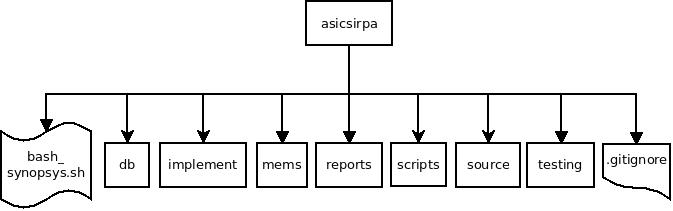
\includegraphics[width=\textwidth]{estructura_1.jpeg}
\centering
\caption{Esquema de la jerarquía de directorios y archivos para implementar el flujo de diseño digital. El archivo .gitignore es un archivo oculto, contiene información para que el sistema de control de versiones opere de forma personalizada, carece de relevancia para la estructura del flujo; sin embargo, permite mantener un repositorio más ordenado. \cite{website:gitignore, website:cvs}}
\label{directorios}
\end{figure}

Como puede apreciarse en la figura \ref{directorios} el directorio base del proyecto contiene hasta el momento siete directorios y dos archivos, uno de los cuales es oculto y carece de relevancia para el proyecto. Comenzando por el archivo \textbf{bash\_synopsys.sh}, tenemos un script de bash, que es una de las tantas consolas que ofrecen los ambientes linux, este script contiene punteros hacia los archivos ejecutables del juego de herramientas de Synopsys, la licencia para que puedan correr, y finalmente cualquier otro software a fín al proyecto pueda ser usado.

Dentro de la estructura propuesta existe un archivo que es importante para que el flujo de diseño sea más cómodo para el usuario, el archivo del que se habla es el archivo \textbf{.bashrc}, el cual es un archivo oculto y se ubica en el directorio principal del usuario, a este directorio suele denominarsele como: "HOME", es universal en cualquier computador con un sistema operativo linux moderno. Este archivo es ejecutado cada vez que se abre una terminal o consola de tipo bash, y le permite al usuario personalizar distintos aspectos de la consola, gracias a esta cualidad es posible abrir una terminal y contar con la posibilidad de disponer de las herramientas necesarias sin tener que ejecutar el script "bash\_synopsys.sh" cada vez que se abre una nueva terminal.

Este archivo (.bashrc) también permite crear variables con rutas relativas a directorios. El contexto en el que se establece la premisa de rutas relativas, corresponde a que el proyecto al ser de dimensiones considerables, involucra a varias personas, y entre otras cosas también existe una herramienta para el manejo de versiones "CVS" \cite{website:cvs}, además es probable que existan muchas copias del proyecto en distintos computadores o servidores.

Así, al hablar de rutas relativas se refiere a que cada computador tiene una ruta absoluta diferente hacia el directorio del proyecto, pero, una vez que se encuentre dentro del directorio del proyecto, las rutas hacia directorios y archivos se vuelven iguales para todos los involucrados. Mediante el uso de variables es posible usar un único comando de referencia en los scripts, y usando variables con rutas relativas, permite abstenerse de editar los scripts en cada computador. Más adelante se expondrá un poco más sobre la importancia de las rutas relativas cuando se hable de los scripts para ejecutar los procesos de síntesis. Podemos ver lo expuesto anteriormente en el diagrama de la figura \ref{bash_syn}.

\begin{figure}[h]
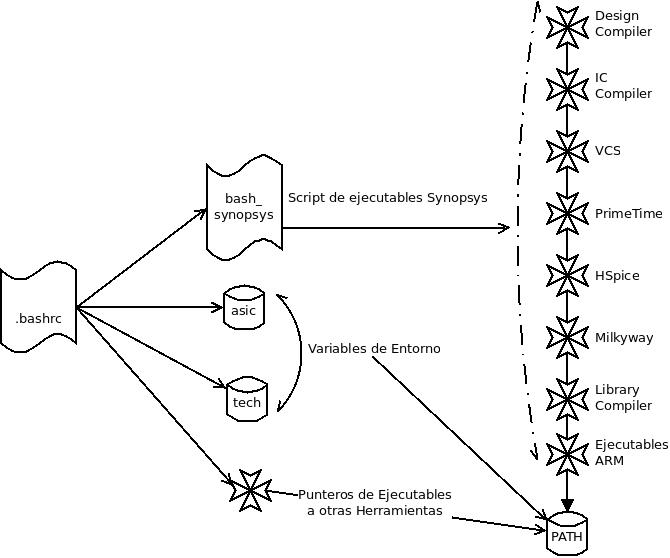
\includegraphics[width=\textwidth]{s_bash.jpeg}
\centering
\caption{Esquema ilustrativo de la relación entre los scripts de bash que inicializan las herramientas EDA y crean las varibles que contienen los punteros a los archivos y la biblioteca de la tecnología de integración}
\label{bash_syn}
\end{figure}

A continuación podemos observar un ejemplo que ilustra, la ejecución del script de bash para incluir en la variable de ambiente "PATH", las rutas a los ejecutables de las herramientas EDA (línea 8), y la creación de 2 variables con la ruta relativa al directorio base del proyecto (variable "asic", línea 3)


\definecolor{mygray}{rgb}{0.5,0.5,0.5}
\definecolor{mygreen}{rgb}{0,0.4,0.1}

 \begin{lstlisting}[language=bash, numbers=left, keywordstyle=\color{blue}, commentstyle=\color{mygreen}]
# Home for working on the SiRPA ASIC Integration Project
asic=/home/rcastro/asicsirpa
export asic
# IBM technology files for the Integration Project (Library)
tech=/home/IBM/TECH
export tech
# Load the EDA Synopsys executables
. $asic/bash_synopsys.sh
# Load a text processor application
PATH=$PATH:/home/tools/sublime_text_3
export PATH
\end{lstlisting}


Retomando el diagrama de la figura \ref{directorios}, dentro del directorio del proyecto de integración encontramos siete directorios, de los cuales db, implement, reports y scripts presentan la misma estructura regular, pues en cada uno de estos directorios encontramos otros 2 directorios llamados be y fe, como podrá intuirse hacen referencia a "back end" y "front end" respectivamente, se decidió usar estas abreviaciones por su simplicidad ya que resumen muy concretamente a que hacen referencia y son muy intuitivas.

El directorio \textbf{db} es una abreviación a "Data Base", que en inglés significa base de datos, y precisamente es en este directorio donde se albergan las bases de datos y demás archivos que son producto de los procesos de síntesis, naturalmente en el subdirectorio fe sólo se almacenan los resultados de la sínteisis lógica de los módulos del proyecto.

El directorio \textbf{implement} alude al proceso de ejecución de las herramientas y los procesos de síntesis, este directorio no contiene archivos de gran relevancia para el proyecto, salvo el directorio \textbf{fe} el cual contiene el archivo oculto, \textbf{.synopsys\_dc.setup}, que es un script de \textit{TCL} con comandos de inicialización y preconfiguración de la herramienta \textit{Design Compiler}, este script es de vital importancia para que la herramienta opere de forma adecuada, más adelante se expondrá un poco más sobre este archivo. Este directorio se emplea para concentrar los archivos temporales que se producen cuando se trabaja con las herramientas de síntesis, los directorios \textbf{work} en fe, el cual contiene archivos que se generan al analizar el código fuente en \textit{HDL}, el directorio \textbf{alib-52} que contiene las bibliotecas producto de la compilación del diseño, esta biblioteca contiene información de caracterización de la biblioteca de la tecnología y sirve para acelerar compilaciones subsecuentes. Finalmente dentro del directorio \textbf{implement} tenemos otro directorio llamado \textbf{mw}, este directorio contiene los reportes y anotaciones de la ejecución de la herramienta \textit{Milkyway}, que es una herramienta de \textit{back end} y podría incluirse en el directorio \textbf{be}; sin embargo, se considera adecuado que esta herramienta tenga un directorio particular para sí, más adelante se explicará la funcionalidad de esta aplicación y el porqué de esta separación.

Siguiendo con los directorios que presentan regularidad, encontramos los directorios: \textbf{reports} y \textbf{scripts}, los cuales contienen reportes y scripts respectivamente. Los reportes generados son distintos de los que genera la herramienta a la hora de estar haciendo el proceso de síntesis, estos reportes corresponden a la información final de síntesis y proveen información útil en la toma de decisiones de las etapas posteriores. Luego los scripts, son los códigos principalmente en lenguaje \textit{TCL} donde se condensan los comandos que usan las herramientas para generar los procesos de síntesis. En el directorio scripts se observan otros dos directorios, \textbf{mw} y \textbf{other}, que contienen respectivamente contienen scripts para la herramienta \textit{Milkyway}, y de otras herramientas como por ejemplo \textit{MATLAB} y los generadores de memorias \textit{SRAM} de \textit{ARM}, los cuales serán expuestos más adelante.

Los tres directorios restantes, \textbf{mems}, \textbf{source}, y \textbf{testing}, no presentan una estructura regular como la que hemos visto hasta el momento, el directorio \textbf{testing} podría incluirse en esa categoría; sin embargo, la subdivisión que presenta es bastante puntual e intuitiva, así que se considera más práctica. Como se puede abstraer "testing", es una palabra en inglés cuya traducción es "pruebas", aquí se alojan los resultados de las distintas simulaciones con las que se valida la funcionalidad de los módulos sometidos al flujo, las simulaciones se subdividen en tres categorías, por comportamiento, en inglés, \textbf{behavioral}, post síntesis lógica (\textbf{post\_syn}), y post síntesis física (\textbf{post\_phy}). Estos tres directorios cuentan con 3 archivos principales, los punteros de compilación, archivos fuente, y un script en \textit{bash} que permiten invocar la herramienta de simulación y ejecutar las compilaciones y simulaciones respectivas, luego de la simulación puede que sea de interés guardar un vector de resultados en un archivo de texto. Así que los directorios de simulación presentan cuatro archivos importantes, los archivos extra que puedan encontrarse en estos directorios son producto de los apuntes y registros que genera la herramienta durante la compilación, y pueden ser obviados.

El directorio \textbf{source}, que se traduce como fuente, contiene dos categorías de directorios, el primero corresponde a los archivos \textit{HDL} con la información modular del diseño, es decir los archivos con la descripción por comportamiento del diseño, y también los archivos con los vectores de estimulos y arreglos o bancos de prueba, es decir los \textit{testbenchs o testfixtures}. Los primeros usados en el proceso de síntesis lógica, y los últimos necesarios para las simulaciones en los distintos dominios.

Por último tenemos el directorio \textbf{mems}, el cual es un directorio bastante particular. Contiene la información producida por los aceleradores de diseño de \textit{ARM}, los cuales generan celdas de memoria \textit{SRAM}. Se trata este proceso aparte ya que los programas para generar las celdas de memoria tienen una metodología de trabajo un poco diferente de la del flujo digital que se ha venido exponiendo. La justificación de manejar estos directorios aparte recae en no mezclar las metodologías de trabajo; sin embargo, el producto final de este procedimiento se integra a la estructura que se ha venido describiendo, es decir se generan bases de datos para las etapas de \textit {back y front end}, posteriormente se ahondará en detalles cuando se expongan los scripts de síntesis de las \textit{SRAM}.

En este directorio (\textbf{mems}), se encuentran dos directorios principales, \textbf{mem\_inst}, el cual contiene los ejecutables de las herramientas de \textit{ARM} para sintetizar las memorias, es importante que sólo exista una única copia de este directorio, ya que es muy pesado (en términos de espacio, cerca de 2 GB), y generaría saturación en un repositorio, que se debe mantener simple y con la menor densidad posible. El otro directorio es \textbf{mem\_work}, el cual contiene el resultado de la síntesis de las celdas \textit{SRAM} y finalmente \textbf{vclef} el cual es un archivo con la información de los metales y el enrutado de la celda \textbf{SRAM} física, este último se crea con el fin de facilitar la ejecución de la herramienta \textit{Milkyway} y generar las base de datos necesarias para los procesos de \textit{back end}. Nuevamente esto será discutido en detalle en un apartado posterior.

\section{Scripting}

Como se ha visto, el flujo de diseño digital se divide en dos etapas principales, \textit{front end} y \textit{back end}. En la parte de \textit{fron end}, se establece la siguiente jerarquía de scripting.

\subsection{Scripts de Front End}

En la figura \ref{s_syn} se observa como la síntesis lógica se ejecuta mediante tres scripts, dos de los cuales son auxiliares al script de síntesis, los scripts se nombran de acuerdo con un nombre representativo del diseño con el que se trabaja, aunque suele ser conveniente nombrar los archivos de la misma manera al módulo principal, si este nombre es muy largo, es preferible optar por un nombre representativo.

\begin{figure}[h]
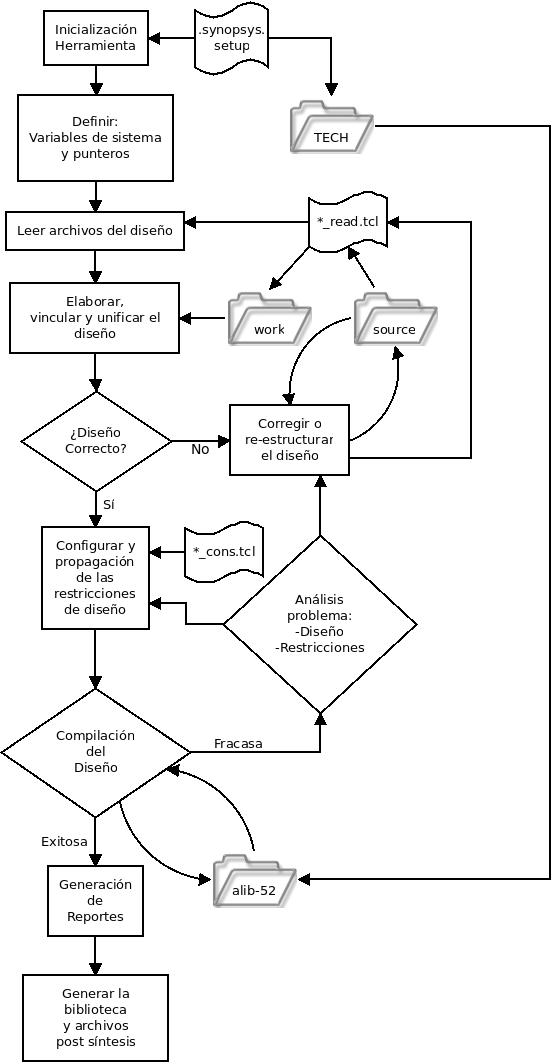
\includegraphics[scale=0.55]{log_syn.jpeg}
\centering
\caption{Diagrama de flujo del scripting que ejecuta la síntesis lógica}
\label{s_syn}
\end{figure}



Es aconsejable separar las instrucciones de síntesis de la herramienta para no generar scripts densos en código y modular las operaciones ejecutadas por la herramienta.

Existe un único flujo en la ejecución de los scripts. El script principal, (*\_syn.tcl) contempla el diagrama de la figura \ref{s_syn}, a partir de la etapa en la que se definen los punteros y las variables del sistema, continúa en línea recta hasta la generación de la base de datos y demás archivos post síntesis. En un apartado anterior se mencionó sobre la importancia del script \textbf{.synopsys\_dc.setup}, este archivo contiene comandos y procedimientos de \textit{TCL} que ejecutan tareas configuración, tal como inicialización de parámetros y variables, declaración de las bibliotecas de diseño.

Cuando la herramienta \textit{Design Compiler} es invocada, ésta busca el archivo configuración en la dirección desde dónde fue invocada, al leer los archivos la herramienta tendrá la información de la ruta hacia las bibliotecas, y cualquier otra personalización que el usuario considere necesaria para facilitar el uso de la herramienta, como crear un alias para comandos en particular, definir la ruta del directorio \textit{alib-52}, el cual se usa para sintetizar una biblioteca reducida y acelerar el proceso de compilación lógica, aunque este es un directorio que le facilita la operación a la herramienta, y las bibliotecas generadas pueden ser utilizadas en etapas posteriores del diseño, no es imperativo que este directorio permanezca en el proyecto, y tampoco es imperativo incluirlo en un repositorio, ya que versionarlo carece de sentido práctico.

Otro de los usos más significativos que se le da al archivo \textbf{.synopsys\_dc.setup} en este proyecto es adquirir variables del sistema operativo para definir variables locales al entorno de la herramienta, estas consisten consiste en rutas relativas al directorio base del proyecto y el directorio base de la biblioteca de la tecnología.

Crear este tipo de variables facilita que los scripts puedan parametrizarse y estos sean capaces de ser usados en distintos equipos sin tener que alterarlos o acondicionarlos significativamente, para que puedan ser funcionales independiente a las rutas locales de los archivos en otros equipos.

Cabe destacar que no toda la configuración de parámetros y variables se realiza en este archivo, y aunque es posible, tampoco es eficiente hacerlo. Este archivo tiene un caráter más genérico. Su función es poner la herramienta a punto para que este en capacidad de sintetizar correctamente cualquier diseño. Las particularidades de los diseños que se trabajan son contempladas en el script de restricciones (constraints), así que no todas las restricciones de diseño se incluyen en este script, sólo las que son universales para cualquier diseño. 

Una vez que la herramienta ha sido inicializada, se procede a configurar variables y parámetros propios del diseño con el que se trabaja. Estos son principalmente variables de rutas hacia el destino de los archivos de salida, y reportes, así como punteros hacia la ruta a bibliotecas auxiliares para el diseño en particular. Así también se crean variables con el nombre del proyecto para que al generar los archivos de salida se usen los comandos de forma paramétrica. Es decir los comandos dependen del valor o contenido de las varibles, esto último se realiza con la finalidad de tener un script genérico, al cual se le deba dar una edición mínima cuando deba ser adaptado a otro diseño.

\subsubsection{Script de lectura de archivos fuente}

Cuando finalmente se han definido todos los parámetros y variables generales para el diseño particular con el que se trabajará, se procede a leer los archivos fuente del diseño, esto corresponde a los módulos descritos en \textit{HDL}. La herramienta debe analizar cada archivo, dependiendo del proyecto pueden existir una enorme cantidad de módulos por analizar, esta es la razón por la que se genera un script de lectura de módulos.

Usando las ventajas de los lenguajes compilados como lo es \textit{TCL}, la lectura y análisis de los módulos se puede realizar de forma programática. En el script \textbf{*\_read.tcl} se usa una variable con el puntero hacia el directorio base de los archivos \textit{HDL} fuente, luego mediante una subrutina de \textit{TCL} se crea una colección con los directorios que contienen los distintos módulos posteriormente se ejecuta un pequeño algoritmo recursivo que recorre las colección de los directorios, para cada directorio se crea otra colección con los módulos, los cuales nuevamente son leídos de manera recursiva. Al recorrer esta última colección se ejecuta el comando de análisis de la herramienta, así se analizan todos los módulos del diseño de forma automática, sin tener la necesidad de incluir en el script la misma instrucción repetida para leer cada posible archivo del proyecto.

\begin{figure}[h]
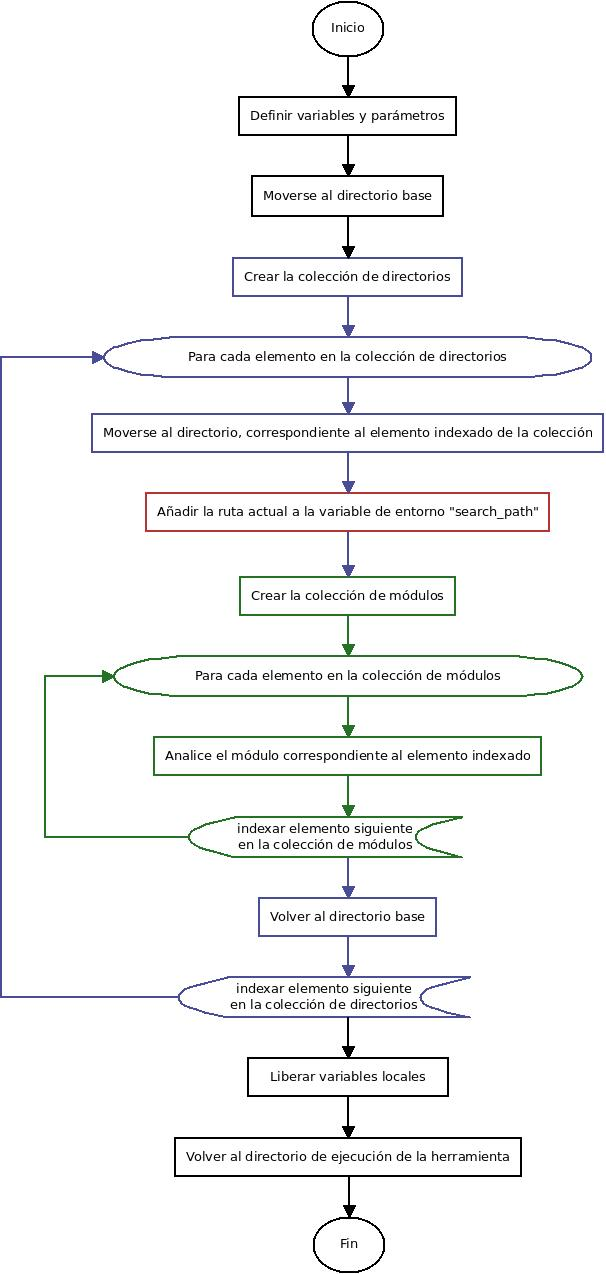
\includegraphics[scale=0.45]{read_script.jpeg}
\centering
\caption{Algoritmo recursivo de lectura y análisis de los módulos \textit{HDL} del diseño}
\label{s_read}
\end{figure}

En la figura \ref{s_read} se observa un diagrama de flujo, con el resumen gráfico del algoritmo descrito en los párrafos anteriores, cabe destacar que en el bloque que indica la definición de variables y parámetros hace referencia a variables locales para ejecutar las tareas de lectura, aunque en realidad únicamente se crean punteros (a los que también llamaremos variables de ruta) hacia las rutas base de los archivos fuente.

Cabe destacar que para algunos diseños, las variables de ruta no necesariamente apuntan a directorios con contenido \textit{HDL}, pues como suele hacerse en proyectos muy grandes, conviene dividir el diseño general en subdiseños más compactos, esto último implica que para algunos proyectos es preferible leer las bases de datos generadas para otros diseños, pues es más práctico.

Otra observación que se debe realizar al diagrama de la figura \ref{s_read} es que no en todos los diseños es necesario crear una colección de directorios, pues si todos los archivos fuente de ese diseño se concentran en un directorio, recorrer la colección de directorios carece de sentido. Consecuentemente puede omitirse el lazo de color púrpura, correspondiente al algoritmo iterativo de indexación de directorios. El único lazo estrictamente necesario para leer los archivos fuente, es el lazo en color verde. Se incluyen ambos lazos en la figura \ref{s_read}, y se expuso el proceso de lectura y análisis con los dos lazos para ilustrar el caso más general de lectura de archivos fuente. Naturalmente los scripts deben ajustarse a la estructura particular del diseño; sin embargo, el algoritmo expuesto es fácilmente adaptable a cada caso.

Siguiendo con la figura \ref{s_read}, y dándole continuidad a la idea expuesta en el párrafo anterior,procede declarar que conviene conservar el bloque de añadir en la variable "search\_path" la ruta actual (bloque en color rojo), ya que al usar el comando de análisis de la herramienta \textit{Design Compiler}, si la ruta relativa al archivo no se ha incluído a la variable de búsqueda (search\_path) la herramienta ofrecerá un error, pues se pretende acceder a una ubicación que no ha sido autorizada para la herramienta.

La variable "search\_path", es una variable propia del entorno de las herramientas de \textit{Synopsys}, su función es manejar una colección de ubicaciones o rutas permitidas para que le herramienta pueda leer y escribir archivos.

Finalmente conviene volver a la ubicación desde donde se ejecutó la herramienta para evitar crear archivos de apuntes, o archivos temporales con poca relevancia para el proyecto, en directorios ajenos a los destinados para esta tarea. Basta decir que liberar todas las variables locales al finalizar una subrutina es una buena práctica de programación, así que es conveniente hacerlo.

Volviendo a la ejecución del script principal de síntesis, cuando ya todos lo módulos son leídos, en el directorio work se crean archivos con información sobre el resultado del análisis de los módulos, de momento estos archivos serán fundamentales para avanzar en el flujo de síntesis, pero una vez acabado el flujo y habiendo generado la base de datos del diseño, no son tan relevantes.


Dicho lo anterior, se debe proceder a elaborar el diseño, esto consiste en definirle a la herramienta cuál es el módulo principal del diseño, posteriormente se deben vincular y unificar todos los módulos. La vinculación y unificación establece la jerarquía modular del diseño y resuelve la interdependencia de los módulos.

En la figura \ref{s_syn} se observa un bloque condicional (diamante de decisión), evaluando la condición si el diseño es correcto. En otras palabras, la herramienta evalúa entre otras cosas, si la semántica del código es correcta, no existen errores sintácticos y todas las dependencias se cumplen. Este bloque condicional no se asocia a una subrutina programática en el script, de hecho ninguno de los bloques condicionales que se aprecian en este diagrama lo hace, en la semántica del flujo también interviene el criterio del diseñador y este es un claro ejemplo de esta situación.

Muy probablemente cuando se le solicite a la herramienta evaluar el diseño, aparecerán mensajes de información, alarmas, y en el peor de los casos, errores. El diseñador entonces, deberá evaluar el escenario con el que se enfrenta, corregir los errores es imperativo; sin embargo, muchos de las alertas son tolerables o inofensivas, así que de acuerdo con la experiencia del diseñador se deberá mejorar o no el diseño, y solucionar o aprobar los mensajes de alerta. ¡Un ingeniero en diseño VLSI, debe aprender a vivir bajo el warning!


Si el diseñador no se siente satisfecho con el resultado de la comprobación de la herramienta, y los mensajes sugieren que debe hacer correcciones a los archivos fuente del diseño, lo más sensato es ponerse en contacto con el departamento o personal encargado del diseño por comportamiento y exponer la situación. En algunos casos el diseñador de \textit{front end} podrá verse arrastrado a analizar y corregir el código fuente, esto suele ser muy raro, ya que las tareas en el flujo de integración suelen estar muy bien definidas de acuerdo con departamentos creados para delimitar y definir tareas y responsabilidades, al menos es así en las industrias de gran envergadura; sin embargo, para diseños de baja envergadura, e instituciones académicas es común encontrar a una única persona realizando todas las tareas relacionadas al flujo.

Cuando la comprobación del diseño es aprobada, lo siguiente es establecer las cotas del comportamiento o dicho de otro modo, las restricciones de operación del diseño y propagarlas por la jerarquía, así todas las dependencias tendrán las mismas condiciones de funcionamiento . Esto quiere decir que se deben definir las condiciones bajo las que el diseño va a operar, como por ejemplo, se definen las características de señales críticas y de alta importancia para el diseño como el reloj.

\subsubsection{Script de restricciones}

En esta etapa es donde se invoca el script de restricciones, en inglés "constraints". Este script se encuentra en el flujo del diagrama de la figura \ref{s_syn} como \textit{*\_cons.tcl}. Para este script no hace falta mostrar un diagrama de flujo sobre su comportamiento ya que en principio sólo define parámetros y variables de entorno de la herramienta \textit{Design Compiler}.

A continuación se presenta un pequeño resumen de los parámetros que se consideran suficientes para cumplir a cabalidad las expectativas de desempeño del diseño.

\begin{itemize}
\item \textbf{Señal de reloj:} {Esta señal necesita en principio ser creada, con esto se refiere a generar un objeto\footnote{Entendiendo por objeto al concepto de programación de alto nivel asociado al ente programático capaz de presentar una colección de atributos y permitirle a funciones complejas invocarle y utilizar sus atributos en tareas específicas. Para más información se invita al lector a que consulte un diccionario sobre terminología en el diseño de software} para que la herramienta pueda crear un árbol de reloj hacia los módulos sincrónicos del diseño. Debe definirse un nombre representativo para la señal en el diseño, hay que recalcar que es conveniente definir una nomenclatura estándar para un proyecto grande que involucre diseños jerarquizados, así cada subdiseño tendrá una señal de reloj con las mismas propiedades y un mismo nombre.

Una vez se crea el objeto "señal de reloj", se definen sus propiedades, en esencia, se define el periodo, la incertidumbre y la latencia de la señal, siempre asociando cada propiedad al objeto "señal de reloj" que ha sido creado. Pueden definirse más propiedades, o las mismas de formas diferentes ya que la herramienta lo permite, pero se considera que estas son suficientes.}

\item \textbf{Propagación de señales:} {Cuando se tienen señales universales a todos los módulos secuenciales, como lo suelen ser las señales de reloj, reset (reinicio), enable (habilitación), preset (preconfiguración), etc. Es posible y es conveniente definir condiciones de comportamiento para la herramienta, ya que esta suele hacer cosas indeseables como colocar buffers en el camino de propagación de señales críticas. Una compuerta lógica, como lo es un buffer presentará efectos de retardo de propagación, lo cual a posteriori se traduce en problemas de sincronización. Es por ello que para estas señales se define un atributo para que la herramienta no realice optimizaciones en ellas. Y el diseñador tendrá un mejor control sobre lo que suceda con esas señales. En este caso únicamente la señal de reloj y reset se definen como intocables.}

\item \textbf{Comportamiento de otras señales:} {Para generar de forma adecuada los modelos simulación, y hacer estimaciones certeras sobre la sincronización de las señales, es beneficioso definir los retardos de propagación de entrada y salida de todas las señales, excepto las mencionadas anteriormente (reloj y reset). Los estímulos en el cableado no se propagan de forma inmediata, por lo que se debe procurar emular un comportamiento cercano a la realidad, para que el resultado de la síntesis del diseño sea lo más confiable posible.}

\item \textbf{Modelo de carga para el cableado:} {Continuando con la idea de generar un modelo lo más realista posible, se deben considerar las características energéticas del cableado.

Conocer las parasitancias de los materiales que se pretenden usar para alimentar e interconectar los módulos del diseño, permite elaborar modelos de comportamiento más cercanos a la realidad. Conocer las propiedades resistivas ayuda a elaborar estimaciones de consumo y desempeño energético, los efectos capacitivos e inductivos permiten evaluar los fenómenos de retardo en las señales, consumo de potencia dinámica, cuando hay conmutación en las señales. Incluso, es posible considerar interferencia por radiación de campos eléctricos y en menor medida los magnéticos. El modelo de cableado o alambrado, es fundamental en sistemas de integración modernos, donde la escala de integración es cada vez más pequeña, a partir de los 300 nm es imperativo contemplar estos efectos.}

\item \textbf{Celdas de conducción:} {El nombre de este atributo, es "driving\_cell", la traducción literal al español no es muy certera; sin embargo, es suficientemente clara. La herramienta necesita que este atributo sea definido para usar una celda adecuada, un buffer, para conectar los módulos del diseño a los puertos de entrada y salida. Esto debe hacerse, en las señales que se propagan hacia puertos de entrada y salida principales e intermodulares.

Una carga excesiva para las señales, suele asociarse a pérdida de información, e inclusive inoperabilidad de algunos segmentos, no se entrará en detalles sobre porqué es importante respetar los fanouts\footnote{El fanout o abanico de salida hace referencia a la máxima cantidad de carga (conexiones) que una señal o puerto es capaz de manejar, hasta que por razones de potencia, esta se empiece a degradar y la señal alcanza niveles de tensión que pueden conducir a la metaestabilidad.} de las señales.

Contemplar las capacidades de conexión de una señal hacia múltiples dependencias, y garantizar la integridad de la información transmitida por dicha señal, es una práctica muy favorable para garantizar la operación exitosa de un diseño. Es por ello que en este apartado también se define un valor máximo de fanout}

\item \textbf{Factor de Actividad:} {El factor de actividad es un parámetro que le indica a la herramienta, como promediar el consumo de potencia dinámico de las señales. En la literatura este parámetro se denomina con la letra griega alfa (\textbf{$\alpha$}).

El factor de actividad, $\alpha$, indica cuantas veces conmuta una señal por ciclo de reloj, naturalmente en un diseño complejo habrán muchas señales con factores de actividad diversos y este cambiará de acuerdo con la tarea que se ejecuta. El valor adecuado a usar en este parámetro responde más a la evidencia empírica y a la experiencia del diseñador.\cite{book:weste2005}

El uso de este parámetro ofrece la posibilidad de generar un reporte de estimación de consumo energético más cercano al comportamiento real del diseño.}
\end{itemize}

Existen muchos otros parámetros que permiten personalizar y condicionar de forma más profunda el diseño, no obstante se expusieron las principales categorías que se deben contemplar y algunas particularidades que se consideran importantes para generar modelos suficientemente cercanos a la realidad. La selección de parámetros suele ser hecha por los ingenieros que se definen los alcances y el desempeño esperado del diseño.

Una vez que las restricciones de diseño han sido definidas y propagadas. Se procede a compilar el diseño, que es la esencia de la síntesis lógica. La compilación le indica a la herramienta que debe generar un nuevo proyecto usando las celdas estándar de la biblioteca de la tecnología, e implementar la estructura abstraída del modelo por comportamiento analizado. En resumen a partir del resultado del análisis del diseño en \textit{HDL} se crea una nueva estructura que mantiene la jerarquía de las funciones y tareas, pero estas ya no se implementan mediante código \textit{HDL} si no mediante elementos de circuitos digitales. En la figura \ref{comp} se observa una analogía gráfica de lo expuesto anteriormente.

\begin{figure}[h]
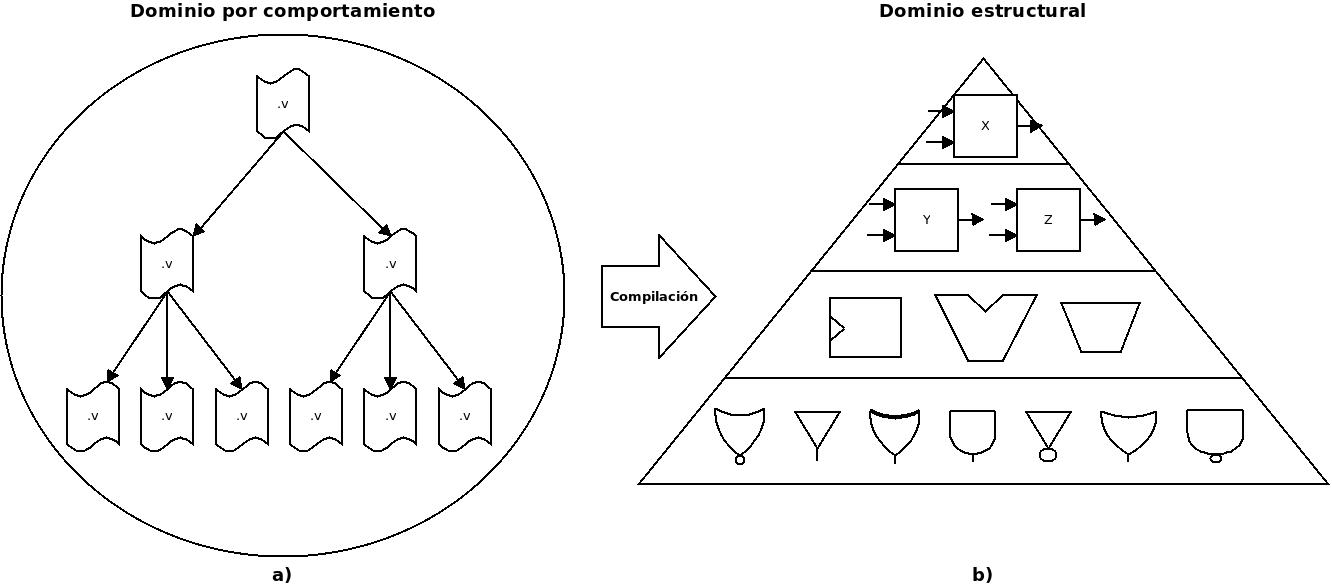
\includegraphics[width=\textwidth]{Compile.jpeg}
\centering
\caption{Ilustración del proceso de compilación. En figura \textbf{$a)$} se aprecia la estructura jerárquica de códigos en \textit{HDL}, y en la figura \textbf{$b)$} la jerarquía abstraída, implementada mediante distintos niveles de elementos digitales, pasando desde funciones complejas, módulos digitales avanzados, hasta compuertas lógicas fundamentales.}
\label{comp}
\end{figure}

Retomando la figura \ref{s_syn} recordamos que el bloque de compilación nuevamente es representado por un diamante de decisión, este diamante no refiere a un evento programático, si no a una etapa en la que el diseñador deberá evaluar si la compilación del diseño es satisfactoria. En esencia la compilación se corrobora mediante la solicitud de reportes a la herramienta, en este punto las bibliotecas compiladas en el directorio \textit{alib-52} y los alias creados en el script de inicialización son bastante útiles, ya es posible repetir el procedimiento de compilación con relativa facilidad y rapidez.

Es conveniente desviar los resultados de la síntesis (compilación) hacia archivos, para mantener un registro. Esto permite llevar un registro del comportamiento de los diseños, y en caso de que se deba se podrá consultar el resultado de un proyecto anterior, para así evaluar si de ser necesario incluirlo en otro proyecto, ese proyecto anterior cumple las expectativas para el nuevo diseño.

La herramienta permite generar reportes de:

\begin{itemize}
\item \textbf{Sincronización (timing):} {Consiste principalmente en la tabulación de la información asociada a la propagación de la señal de reloj del circuito. Es un análisis que estima el retardo en el diseño basándose únicamente en la topología de las rutas de propagación de la señal de reloj.

A lo anterior se le conoce como \textbf{esfuerzo lógico}, por lo tanto la solicitud de este reporte a la herramienta, consigue un analisis de esfuerzo lógico en el diseño. La herramienta genera entonces un presupuesto teórico de cuanto debe tomarle a la señal, el propagarse a través de una determinada ruta, y evaluar, junto con la información suministrada por las restricciones del diseñador, y la información que aporta la biblioteca de la tecnología, si los datos llegan en el tiempo presupuestado, conocido como "slack MET"\footnote{Es posible ahondar más sobre qué es el "slack" y cual es su relevancia; sin embargo, este informe pretende desvelar el flujo de diseño digital. Se parte de la premisa que el lector comprende el uso de términos como: slack, hold time o setup time, hablar más al respecto está fuera del objetivo de este informe.}.}

\item \textbf{Potencia:} {Se refiere a una descripción resumida de las características de alimentación del diseño, esto se refiere a la tensión nominal de operación general de los dispositivos, el comportamiento estático y dinámico de las celdas estándar en términos de disipación energética. La información aparece resumida y tabulada, de forma que se puede encontrar cuanta energía se disipa o consume en un bloque en particular, entiéndase por bloque, los dispositivos combinacionales, secuenciales, señales, etc. }

\item \textbf{Área:} {Este reporte es un pequeño resumen del volumen o cantidad de celdas usadas (combinacionales y sequenciales), celdas extra como buffers, señales y puertos. Se hace una recopilación de el espacio que se preveé será necesario para colocar estos elementos en el espacio del dado de silicio, en etapas posteriores. La información más útil es que permite tener una idea del área necesaria para la colocación cuando deba diseñarse el floorplan, y le permite al diseñador efectuar un buen ansatz\footnote{Anzats: término de origen alemán, usado comúnmente por físicos y matemáticos para referirse a una estimación que permite resolver una ecuación o un problema. Refiérase a un diccionario de alemán.} al definir el tamaño del plano de colocación y enrutado (floorplan) del diseño durante la implementación física.}

\item \textbf{Celdas:} {Consiste en un listado de las celdas estándar necesarias para implementar el diseño. Se presenta en forma tabular, describiendo el nombre de referencia de la celda, el bloque de diseño donde es usada, el área que ocupa, y en que biblioteca donde se encuentra. Es útil para generar bibliotecas reducidas que permiten compilaciones más rápidas, y le permite al diseñador saber cuales bibliotecas debe tener en cuenta al hacer la implementación física o deba hacer simulaciones.}


\item \textbf{QOR (Quality of Results):} {Se traduce como calidad de resultados y es un compendio de varios de los atributos que se exponen en los otros reportes, tiene información sobre el área, la naturaleza de las celdas usadas, los caminos críticos de retardo, así como violaciones de sincronización, violaciones de reglas de diseño, inclusive presenta estadísticas del desempeño del computador que corrió la herramienta de síntesis. Se puede afirmar que es un resumen muy general del trabajo hecho en la síntesis del diseño.}
\end{itemize}

Finalmente es necesario guardar el proyecto y generar archivos que permitan evaluar si el proyecto cumple las expectativas de comportamiento, (ejecuta las funciones para las que fue concebido), y generar los archivos que permiten continuar el flujo de diseño. En resumen de lo anterior, se deben generar los archivos que tienen la información del resultado del proceso que se acaba de realizar, además generar los modelos para evaluar si los resultados siguen cumpliendo las expectativas de funcionamiento establecidas.

Los principales archivos generados son los siguientes:

\begin{itemize}
\item \textbf{DDC:} {Este es un archivo jerárquico, el cual define la estructura del diseño, qué celdas son necesarias para implementarla, todas las dependencias entre éstas, además de información de conectividad para implementar el comportamiento abstraído del diseño \textit{HDL}. Este archivo funciona como una base de datos que contiene toda la información expuesta en los reportes. Este archivo es el estándar almacenamiento de la información post síntesis lógica de la herramienta \textit{Design Compiler}, es usado si en un futuro se necesita volver al diseño, ya sea para editarlo o recuperar información, como puede ser generar un reporte, etc. A partir de este archivo se puede continuar con la implementación física.}

\item \textbf{HDL:} {Este código HDL, que para fines prácticos en este informe consiste en códigos \textit{verilog}, se generá es considerablemente diferente del usado anteriormente, pues para la etapa de analisis del proyecto partíamos de un código fuente que describía el comportamiento del diseño, mediante un lenguaje de alto nivel. \textit{Verilog} ofrece la posibilidad de usar funciones de alto nivel para emular el comportamiento de los dispositivos digitales.

\textit{Verilog} también ofrece la posibilidad de implementar circuitos digitales mediante primitivas. Esto se refiere a que puede usar referencias a componentes digitales e interconectarlos de acuerdo con la semántica abstraída del código por comportamiento. A esta forma de codificación se le conoce como \textbf{GLD}\footnote{GLD, o GL refiere a Gate Level Description, en español, Descripción a Nivel de Compuertas. Este concepto refiere a una metodología de descripción de circuitos digitales, que permite establecer la relación entre componentes digitales, y enlazarlos de manera en que se forma una función o circuito más complejo.}

Es conveniente generar 2 archivos con la información del \textit{GLD}, esto con el fin de tener un archivo, que podrá ser usado por la siguiente etapa para iniciar la implementación física, y otro archivo para realizar la simulación post síntesis. La separación se debe a que el archivo que se use para la simulación necesita de una directiva adicional para leer el archivo que provee la información de los retardos, la presencia de esta directiva entra en conflicto con las herramientas de \textit{back end}, de esto se hablará más adelante. Sobra decir que conviene distinguir con un nombre adecuado ambos archivos, en este proyecto se usa la nomenclatura \textit{*\_syn\_sim.v} para diferenciar al archivo de simulación.}

\item \textbf{SDF:} {}

\item \textbf{SDC:} {}

\end{itemize}

\subsection{Simulación Lógica: evaluación post síntesis lógica}

Los reportes generados permiten 